\documentclass{ximera}

\input{../preamble.tex}
\title[Prerequisite Videos: ]{Compositions of Functions}
\author{Ben Sencindiver}

\outcome{Understand function operations, specifically composition of functions.}

\begin{document}
\begin{abstract}
  In this set of videos, we will work to understand
  composition of functions, including evaluation 
  of composition of functions through function 
  notation and graphs, building compositions of functions
  recognition a function composites.
\end{abstract}
\maketitle

The following videos will cover topics about composition of functions:

%% Introduction and Question 1
\textbf{Introduction and Question 1: Definition 
  of composition of functions and  evaluation}
\begin{question}
%% Labeling this expandable option
\begin{flushright}
{\color{blue}(\emph{Click the arrow to the right to see the Introduction video and first question.})}
\end{flushright}
\begin{center}
\begin{expandable}
\youtube{a1xVVhewWFA}
%% Multiple Choice Question 1
{\color{blue}(\emph{Click the arrow to the right to see the question
posed at the end of the video.})}
\begin{expandable}
For $f(x) = x^2 + 1$ and $g(x) =2x-4$, what is $(g \circ f)(2)$?\\
\begin{prompt}
\[
(g\circ f)(2) \text{ is exactly }\answer[given]{6}
\]
\end{prompt}
%% Example 1
\begin{flushright}
{\color{blue}(\emph{Click the arrow to the right to see an example.})}
\end{flushright}
\begin{expandable}
Example 1
\youtube{ezaMDoFfvTE}
\end{expandable}
\end{expandable}
\end{expandable}
\end{center}
\end{question}


%% Question 2
\textbf{Question 2: Evaluation of compositions
of functions via graphs.}
\begin{question}
%% Labeling this expandable option
\begin{flushright}
{\color{blue}(\emph{Click the arrow to the right to see the second question.})}
\end{flushright}
\begin{center}
\begin{expandable}
\youtube{i9KsZxIPQSU}
%% Multiple Choice Question 2
{\color{blue}(\emph{Click the arrow to the right to see the question
posed at the end of the video.})}
\begin{expandable}
\begin{center}
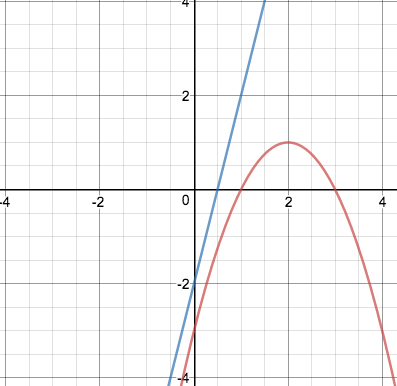
\includegraphics[scale=0.3]{CompFuncGraph1.png}\\
\end{center}
Given the graphs of the functions {\color{red} $f(x)$}
and {\color{blue} $g(x)$} below, what is
$({\color{red} f} \circ {\color{blue} g})(1)$?\\
\begin{center}
\end{center}
\begin{prompt}
\[
({\color{red} f} \circ {\color{blue} g})(1) \text{ is exactly }\answer[given]{1}
\]
\end{prompt}
%% Example 2
\begin{flushright}
{\color{blue}(\emph{Click the arrow to the right to see an example.})}
\end{flushright}
\begin{expandable}
Example 2
\youtube{zPBULCxYa94}
\end{expandable}
\end{expandable}
\end{expandable}
\end{center}
\end{question}



%% Question 3
\textbf{Question 3: Recognizing the pieces of composite functions.}
\begin{question}
%% Labeling this expandable option
\begin{flushright}
{\color{blue}(\emph{Click the arrow to the right to see the second question.})}
\end{flushright}
\begin{center}
\begin{expandable}
\youtube{fZQC7IxOVho}
%% Multiple Choice Question 3
{\color{blue}(\emph{Click the arrow to the right to see the question
posed at the end of the video.})}
\begin{expandable}
Consider the function $h(x) = (x + 1)^2$. If $h(x) = (f\circ g)(x)$ where $g(x) = x+1$ and $f(x)$ is unknown, what is $f(x)$ if $h(x) = (f \circ g)(x)$?\\
\begin{prompt}
\[
\text{The function }f(x) \text{ is exactly }\answer[given]{x^2}
\]
\end{prompt}
%% Example 3
\begin{flushright}
{\color{blue}(\emph{Click the arrow to the right to see an example.})}
\end{flushright}
\begin{expandable}
Example 3
\youtube{l6cbnPH3u9o}
\end{expandable}
\end{expandable}
\end{expandable}
\end{center}
\end{question}


%% Question 4
\textbf{Question 4: Determining pieces of a composite function.}
\begin{question}
%% Labeling this expandable option
\begin{flushright}
{\color{blue}(\emph{Click the arrow to the right to see the second question.})}
\end{flushright}
\begin{center}
\begin{expandable}
\youtube{pPb4zFAREE4}
%% Multiple Choice Question 4
{\color{blue}(\emph{Click the arrow to the right to see the question
posed at the end of the video.})}
\begin{expandable}
Consider the function $h(x) = x^2 + 4x - 7$. If $h(x) = (f\circ g)(x)$
where $g(x) = x+1$ and $f(x) = ax^2 + bx + c$ for some values $a,b,$
and $c$, what is $a, b,$ and $c$ if $h(x) = (f\circ g)(x)$?\\
\begin{prompt}
\[
a = \answer[given]{1}
\]
\[
b = \answer[given]{2}
\]
\[
c = \answer[given]{-3}
\]
\end{prompt}
%% Example 4
\begin{flushright}
{\color{blue}(\emph{Click the arrow to the right to see an example.})}
\end{flushright}
\begin{expandable}
Example 4
\youtube{nYZO4rxM0K4}
\end{expandable}
\end{expandable}
\end{expandable}
\end{center}
\end{question}

\end{document}
